\documentclass{article}

\usepackage{fancyhdr}
\usepackage{extramarks}
\usepackage{amsmath}
\usepackage{amsthm}
\usepackage{amsfonts}
\usepackage{tikz}
\usepackage[plain]{algorithm}
\usepackage{algpseudocode}
\usepackage{listings}
\usepackage{color}
\usepackage{hyperref}
\usepackage{graphicx}

\definecolor{dkgreen}{rgb}{0,0.6,0}
\definecolor{gray}{rgb}{0.5,0.5,0.5}
\definecolor{mauve}{rgb}{0.58,0,0.82}

\lstset{frame=tb,
  language=Java,
  aboveskip=3mm,
  belowskip=3mm,
  showstringspaces=false,
  columns=flexible,
  basicstyle={\ttfamily},
  numbers=none,
  numberstyle=\tiny\color{gray},
  keywordstyle=\color{blue},
  commentstyle=\color{dkgreen},
  stringstyle=\color{mauve},
  breaklines=true,
  breakatwhitespace=true,
  tabsize=3
}

\usetikzlibrary{automata,positioning}

%
% Basic Document Settings
%

\topmargin=-0.45in
\evensidemargin=0in
\oddsidemargin=0in
\textwidth=6.5in
\textheight=9.0in
\headsep=0.25in

\linespread{1.1}

\pagestyle{fancy}
\lhead{\hmwkAuthorName}
\chead{\hmwkClass}
\rhead{\hmwkTitle}
% \rhead{\firstxmark}
\lfoot{\lastxmark}
\cfoot{\thepage}

\renewcommand\headrulewidth{0.4pt}
\renewcommand\footrulewidth{0.4pt}

\setlength\parindent{0pt}

%
% Create Problem Sections
%

\newcommand{\enterProblemHeader}[1]{
  % \nobreak\extramarks{}{Problem \arabic{#1} continued on next page\ldots}\nobreak{}
  % \nobreak\extramarks{Problem \arabic{#1} (continued)}{Problem \arabic{#1} continued on next page\ldots}\nobreak{}
}

\newcommand{\exitProblemHeader}[1]{
  % \nobreak\extramarks{Problem \arabic{#1} (continued)}{Problem \arabic{#1} continued on next page\ldots}\nobreak{}
  \stepcounter{#1}
  % \nobreak\extramarks{Problem \arabic{#1}}{}\nobreak{}
}

\setcounter{secnumdepth}{0}
\newcounter{partCounter}
\newcounter{homeworkProblemCounter}
\setcounter{homeworkProblemCounter}{1}
% \nobreak\extramarks{Problem \arabic{homeworkProblemCounter}}{}\nobreak{}

%
% Homework Problem Environment
%
% This environment takes an optional argument. When given, it will adjust the
% problem counter. This is useful for when the problems given for your
% assignment aren't sequential. See the last 3 problems of this template for an
% example.
%
\newenvironment{homeworkProblem}[1][-1]{
  \ifnum#1>0
  \setcounter{homeworkProblemCounter}{#1}
  \fi
  \section{Problem \arabic{homeworkProblemCounter}}
  \setcounter{partCounter}{1}
  \enterProblemHeader{homeworkProblemCounter}
  }{
  \exitProblemHeader{homeworkProblemCounter}
}

%
% Homework Details
%   - Title
%   - Due date
%   - Class
%   - Section/Time
%   - Instructor
%   - Author
%

\newcommand{\hmwkTitle}{Lab\ \#1}
\newcommand{\hmwkDueDate}{February 12, 2016}
\newcommand{\hmwkClass}{Algorithms and Complexity (DD2352)}
\newcommand{\hmwkAuthorName}{Dhirendra Kholia}

%
% Title Page
%

\title{
  \vspace{2in}
  \textmd{\textbf{\hmwkClass:\ \hmwkTitle}}\\
  \normalsize\vspace{0.1in}\small{Due\ on\ \hmwkDueDate\ at 1:00pm}\\
  % \vspace{0.1in}\large{\textit{\hmwkClassInstructor\ \hmwkClassTime}}
  % \vspace{0.1in}\large{\textit{\ \hmwkClassTime}}
  \vspace{3in}
}

\author{\textbf{\hmwkAuthorName, 850227-8255, kholia@kth.se}}
\date{}

\renewcommand{\part}[1]{\textbf{\large Part \Alph{partCounter}}\stepcounter{partCounter}\\}

%
% Various Helper Commands
%

% Useful for algorithms
\newcommand{\alg}[1]{\textsc{\bfseries \footnotesize #1}}

% For derivatives
\newcommand{\deriv}[1]{\frac{\mathrm{d}}{\mathrm{d}x} (#1)}

% For partial derivatives
\newcommand{\pderiv}[2]{\frac{\partial}{\partial #1} (#2)}

% Integral dx
\newcommand{\dx}{\mathrm{d}x}

% Alias for the Solution section header
\newcommand{\solution}{\textbf{\large Solution}}

% Probability commands: Expectation, Variance, Covariance, Bias
\newcommand{\E}{\mathrm{E}}
\newcommand{\Var}{\mathrm{Var}}
\newcommand{\Cov}{\mathrm{Cov}}
\newcommand{\Bias}{\mathrm{Bias}}

\begin{document}

\maketitle

\pagebreak

\begin{homeworkProblem}
  % http://www.csc.kth.se/~karlan/AoK/Lab_1.html
  % https://en.wikipedia.org/wiki/Levenshtein_distance#Definition
  % http://www.csse.monash.edu.au/~lloyd/tildeAlgDS/Dynamic/Edit/
  Formulate the recursion (partDist in the program) as compact as possible with mathematical notation.

  \lstinputlisting[language=Java]{partDist.java}

  \textbf{Solution}

  \vspace{1em}

  The recurrence relations corresponding to the "partDist" function are,

  \begin{align*}
    partDist(A,B,m,n) = min
    \begin{cases}
      partDist(A,B,m-1,n-1) + 1_{(A_{m-1} \neq B_{n-1})} \\
      partDist(A,B,m,n-1) + 1 \\
      partDist(A,B,m-1,n) +1  \\
      \\
      \begin{cases}
        partDist(A,B,m,n) = m, \ if \ n = 0 \\
        partDist(A,B,n,n) = n, \ if \ m = 0
      \end{cases}
    \end{cases}
  \end{align*}

  Where, \\ \\
  A = w1 \\
  B = w2 \\
  m = w1len \\
  n = w2len

\end{homeworkProblem}

\pagebreak

\begin{homeworkProblem}
  Calculate partDist("labd", "blad", x, y) for all x and y between 0 and 4 and
  enter the results in a matrix M. What is M?

  % http://www.let.rug.nl/~kleiweg/lev/
  % http://www.kurzhals.info/static/samples/levenshtein_distance/

  \vspace{1em}
  \textbf{Solution}
  \vspace{1em}

  % https://www.clear.rice.edu/comp130/12spring/editdist/
  % "labd" forms the rows, while "blad" is along the columns
  \begin{table}[ht]
    \centering
    \begin{tabular}{c | c | c | c | c | c}
      & \(\epsilon\)
      & \(b\)
      & \(l\)
      & \(a\)
      & \(d\)
      \\
      \hline
      \(\epsilon\) & 0 & 1 & 2 & 3 & 4 \\
      \(l\) & 1 & 1 & 1 & 2 & 3 \\
      \(a\) & 2 & 2 & 2 & 1 & 2 \\
      \(b\) & 3 & 2 & 3 & 2 & 2 \\
      \(d\) & 4 & 3 & 3 & 3 & 2 \\
    \end{tabular}
  \end{table}

  M matrix holds the edit distance values. The value M[i][j] represents the
  edit distance between the first i characters of string A and the first j
  characters of string B. The edit distance between "labd" and "blad" is
  given by M[4][4].

\end{homeworkProblem}

\begin{homeworkProblem}
  What does the method partDist(w1, w2, x, y) compute?

  \vspace{1em}
  \textbf{Solution}
  \vspace{1em}

  partDist(w1, w2, xy, y) computes the edit distance between the first x
  characters of string w1, and the first y characters of string w2. E.g
  partDist("labd", "blad", 4 ,4) returns 2, which implies that two
  operations are required to change "labd" to "blad". \\

  The possible operations are replace, delete, and insert.

\end{homeworkProblem}

\begin{homeworkProblem}
  % O(n) represents upper bound. Θ(n) means tight bound. Ω(n) represents lower bound.
  % f(x) = Θ(g(x)) iff f(x) = O(g(x)) and f(x) = Ω(g(x))
  Show that the time complexity of Distance(w1, w2) is \(\Omega(2^{max(n,m)})\) in the
  worst case, where n is the number of letters in w1 and m is the number of
  letters in w2.

  \vspace{1em}
  \textbf{Solution}
  \vspace{1em}

  % http://stackoverflow.com/questions/14616339/complexity-of-edit-distance-levenshtein-distance-recursion-top-down-implementa
  % http://www.geeksforgeeks.org/dynamic-programming-set-5-edit-distance/

    I could not attack this problem completely on my own. I found some help on StackOverflow on \href{http://stackoverflow.com/questions/14616339/complexity-of-edit-distance-levenshtein-distance-recursion-top-down-implementa}{this} page. I also used \href{http://www.geeksforgeeks.org/dynamic-programming-set-5-edit-distance/}{this} GeeksforGeeks article for help. \\

  From solution to problem 1, we have, \\

  T(n,m) = T(n-1,m-1) + T(n-1,m) + T(n,m-1) + C \\
  T(0,m) = m \\
  T(n,0) = n \\

  Where, \\

  n = length(w1) and m = length(w2) \\

  T(n,m) splits into three paths, imagine a picture of a ternary tree where
  T(n,m) represents the root node. \\

  The worst case happens when none of characters of two strings match. Below is
  a non-complete recursive call diagram for the worst case.

  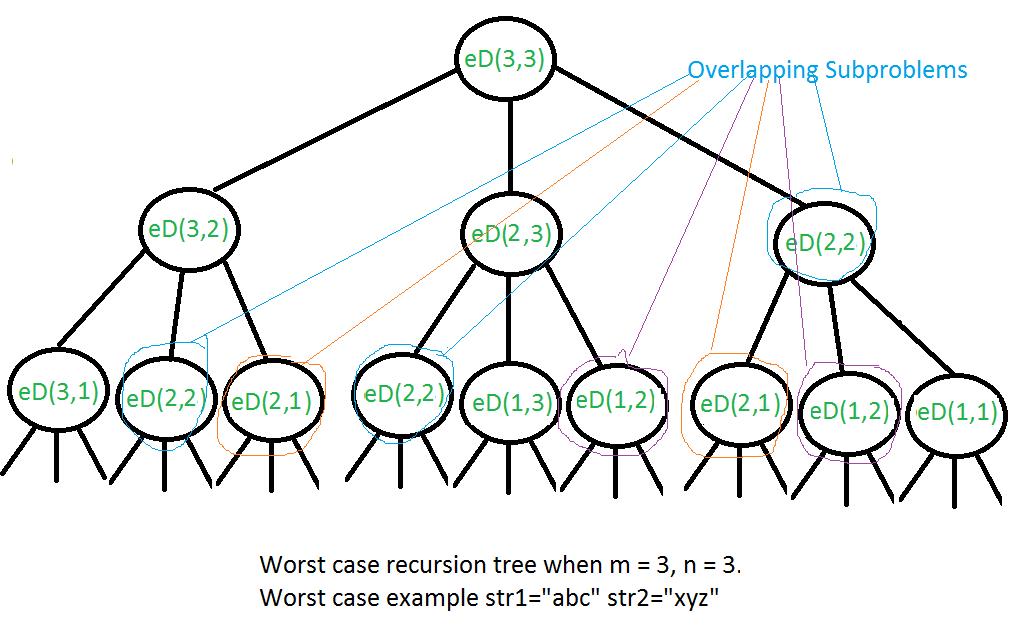
\includegraphics[scale=0.6]{EditDistance}

  The shortest path has the length min(n,m). E.g. if w1 = "ab and w2 = "ab", then
  the shortest path goes from ('ab','ab') to ('a','a') to ('','') which is of
  length 3. Such a ternary tree has at least \(3^{min(m,n)}\) nodes. This is
  the lower bound. \\

  However there are some paths that are longer. The length of the longest path
  is m+n-1. Trace w1 = 'ab' and w2 = 'b' to derive this upper bound (reduce w1,
  and w2 alternatively to prolong the path length). This implies that our
  ternary tree has at most \(3^{m+n-1}\) nodes. This is the upper bound. \\

  % The TA liked our solution this far very much! :-)

  In the worst-case m = n, so \(\Omega(2^{max(n,m)})\) becomes \(\Omega(2^n)\).
  The previously established lower bound \(3^{min(m,n)}\) becomes
  \(\Omega(3^n)\). Since \(\Omega(2^n)\) itself is bounded by \(\Omega(3^n)\)
  it is OK to say that the time complexity of Distance(w1, w2) is
  \(\Omega(2^{max(n,m)})\) in the worst case.

\end{homeworkProblem}

\pagebreak

\begin{homeworkProblem}
  See how you can track the editing operations made in the shortest edit
  sequence from "labd" to "blad" by looking at the matrix M.

  \vspace{1em}
  \textbf{Solution}
  \vspace{1em}

  % http://www.hakank.org/edit_distances/edit_distances.cgi

  Start with x = 4, and y = 4 (the indices of the bottom rightmost element
  which represents the final edit distance). \\

  1. Since A[x] = B[y] (x = 4, y = 4, 'd' is equal to 'd'), no edit operation is
  required. Move diagonally upwards by setting x = 3, and y = 3. \\

  2. A[3] != B[3] ('b' is not equal to 'a') and M[3][3] = 2 which is 1 + M[2][3].
  This implies that A[3] ('b') needs to be deleted. Move up by decrementing x to 2. \\

  3. Since A[2] = B[3] ('a' is equal to 'a'), no edit operation is required. Move
  diagonally upwards by decrementing x and y, x is now 1 and y is 2. \\

  4. Since A[1] = B[2] ('l' is equal to 'l'), no edit operation is required. Move
  diagonally upwards by decrementing x and y, x is now 0 and y is 1. \\

  5. A[0] != B[1] ('' is not equal to 'a') and M[0][1] = 1 which is 1 + M[0][0].
  This implies that B[1] ('b') needs to be inserted at A[0]. Move left by
  decrementing y to 2. \\

  Now x = 0, y = 0 and the algorithm terminates. So in total 2 edits are
  required on the "labd" string, deletion of 'b' (step 2), and insertion of 'b'
  at the start (step 5).

\end{homeworkProblem}

\pagebreak

\begin{homeworkProblem}
  Show with pseudocode how the recursion can be calculated by using dynamic
  programming, i.e. how a matrix M can be created.

  \vspace{1em}
  \textbf{Solution}
  \vspace{1em}

  % https://en.wikipedia.org/wiki/Levenshtein_distance#Iterative_with_full_matrix

  \lstinputlisting[keywords={}]{edit-distance-dp.txt}

  % The TA liked this Python-like pseudocode and said that it is super fine.


\end{homeworkProblem}

\begin{homeworkProblem}
  Analyze the time complexity for determining the editing distance between an
  n-letter word and an m-letter word with dynamic programming.

  \vspace{1em}
  \textbf{Solution}
  \vspace{1em}

  There are (m + 1) * (n + 1) entries in the matrix. Each entry \(M_{ij}\)
  takes O(1) time to calculate. Hence the time complexity for determining the
  editing distance with dynamic programming is \(O(m * n)\).

\end{homeworkProblem}

\pagebreak

\begin{homeworkProblem}
  Calculate the dynamic programming matrix edit distance between "labs" and "blad".

  \vspace{1em}
  \textbf{Solution}
  \vspace{1em}

  \begin{table}[ht]
    \centering
    \begin{tabular}{c | c | c | c | c | c}
      & \(\epsilon\)
      & \(b\)
      & \(l\)
      & \(a\)
      & \(d\)
      \\
      \hline
      \(\epsilon\) & 0 & 1 & 2 & 3 & 4 \\
      \(l\) & 1 & 1 & 1 & 2 & 3 \\
      \(a\) & 2 & 2 & 2 & 1 & 2 \\
      \(b\) & 3 & 2 & 3 & 2 & 2 \\
      \(s\) & 4 & 3 & 3 & 3 & 3 \\
    \end{tabular}
  \end{table}

\end{homeworkProblem}

\begin{homeworkProblem}
  What part of the matrices for "labd" - "blad" and "labs" - "blad" are different?

  \vspace{1em}
  \textbf{Solution}
  \vspace{1em}

  For "labd" - "blad", the edit distance matrix,

  \begin{table}[ht]
    \centering
    \begin{tabular}{c | c | c | c | c | c}
      & \(\epsilon\)
      & \(b\)
      & \(l\)
      & \(a\)
      & \(d\)
      \\
      \hline
      \(\epsilon\) & 0 & 1 & 2 & 3 & 4 \\
      \(l\) & 1 & 1 & 1 & 2 & 3 \\
      \(a\) & 2 & 2 & 2 & 1 & 2 \\
      \(b\) & 3 & 2 & 3 & 2 & 2 \\
      \(d\) & 4 & 3 & 3 & 3 & 2 \\
    \end{tabular}
  \end{table}

  For "labs" - "blad", the edit distance matrix is,

  \begin{table}[ht]
    \centering
    \begin{tabular}{c | c | c | c | c | c}
      & \(\epsilon\)
      & \(b\)
      & \(l\)
      & \(a\)
      & \(d\)
      \\
      \hline
      \(\epsilon\) & 0 & 1 & 2 & 3 & 4 \\
      \(l\) & 1 & 1 & 1 & 2 & 3 \\
      \(a\) & 2 & 2 & 2 & 1 & 2 \\
      \(b\) & 3 & 2 & 3 & 2 & 2 \\
      \(s\) & 4 & 3 & 3 & 3 & 3 \\
    \end{tabular}
  \end{table}

  Only the bottom rightmost entry (2 vs. 3) is different.

\end{homeworkProblem}

\pagebreak

\begin{homeworkProblem}
  Generally, what parts of the matrices for Y-X and Z-X are different when the
  words Y and Z have the same first p letters?

  \vspace{1em}
  \textbf{Solution}
  \vspace{1em}

  Let us denote the length of X by L. \\

  For "labd" - "blad", the edit distance matrix,

  \begin{table}[ht]
    \centering
    \begin{tabular}{c | c | c | c | c | c}
      & \(\epsilon\)
      & \(b\)
      & \(l\)
      & \(a\)
      & \(d\)
      \\
      \hline
      \(\epsilon\) & 0 & 1 & 2 & 3 & 4 \\
      \(l\) & 1 & 1 & 1 & 2 & 3 \\
      \(a\) & 2 & 2 & 2 & 1 & 2 \\
      \(b\) & 3 & 2 & 3 & 2 & 2 \\
      \(d\) & 4 & 3 & 3 & 3 & 2 \\
    \end{tabular}
  \end{table}

  For "laxy" - "blad", the edit distance matrix is,

  \begin{table}[ht]
    \centering
    \begin{tabular}{c | c | c | c | c | c}
      & \(\epsilon\)
      & \(b\)
      & \(l\)
      & \(a\)
      & \(d\)
      \\
      \hline
      \(\epsilon\) & 0 & 1 & 2 & 3 & 4 \\
      \(l\) & 1 & 1 & 1 & 2 & 3 \\
      \(a\) & 2 & 2 & 2 & 1 & 2 \\
      \(x\) & 3 & 3 & 3 & 2 & 2 \\
      \(y\) & 4 & 4 & 4 & 3 & 3 \\
    \end{tabular}
  \end{table}

  The M matrix is same for both cases from M[0][0] to M[p][L]. So only the
  rectangular sub-matrix M[p+1][1] to M[length(Z)][L] is different. \\

  In better words, the rows corresponding to the differing letters are different!

\end{homeworkProblem}

\end{document}
